\chapter{Clasificación de imágenes}

Esta clase tiene como objetivo comprender los conceptos de clasificación espectral y la forma de realizarla en el SNAP utilizando algoritmos de clustering. Para ello clasificaremos una imagen de la zona de la Triple Frontera.

\section{Clasificación por k-means}

Abra la imagen

\begin{center}
\directory{LC08\_224-078\_2018-01-05.dim}.
\end{center}

diríjase luego a \menu{Raster > Classification > Unsupervised classification > K-Means cluster analysis}.

En la pestaña \menu{I/O Parameters} seleccione la imagen que acaba de abrir, junto con el nombre de salida y la carpeta donde guardará la imagen (Figura \ref{fig:kmeans}) y haga click en \menu{Run}.

\begin{figure}[h!]
    \centering
    \subfloat[1-I/O Parameters]{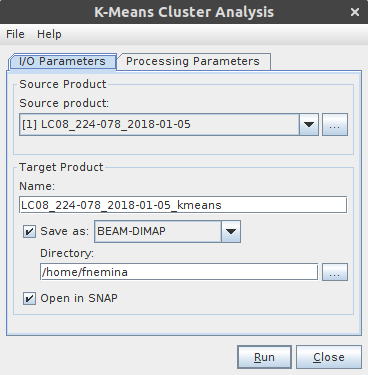
\includegraphics[width=0.4\textwidth]{fig:kmeans1.png}\label{fig:kmeans1}}
    \hspace{1cm}
    \subfloat[Processing parameters]{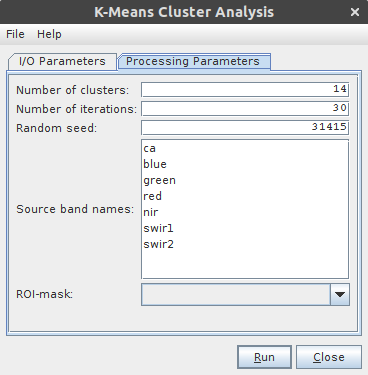
\includegraphics[width=0.4\textwidth]{fig:kmeans2.png}\label{fig:kmeans2}}
    \caption{Clasificación de imágenes por el método \emph{k-means}.}
    \label{fig:kmeans}
\end{figure}

Luego de realizada la clasificación obtendrá una imagen clasificada en el \menu{Product explorer}. Despliegue la banda \menu{class\_indices}.

Es posible ver también los nombres de las clases y el centroide obtenido para cada uno en \emph{Index Codings, Cluster\_classes} dentro de la imagen.

\section{Reclasificación}

La imagen obtenida por el método de clasificación es de clases espectrales. Para obtener una imagen con clases de información es necesario reclasificar los valores asignando nombres y colores a cada clase espectral. Para hacerlo despliegue en simultáneo la imagen clasificada y una combinación de bandas conveniente.

Seleccione la imagen clasificada y haga click en \menu{View > Tool windows > Colour manipulation} (Figura \ref{fig:colman}).

\begin{figure}[h!]
    \centering
    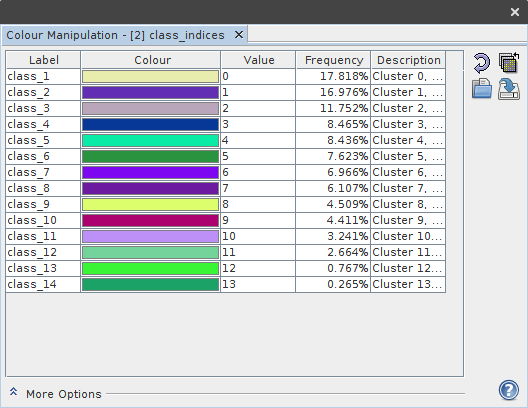
\includegraphics[width=0.4\textwidth]{fig:colman.png}
    \caption{Herramienta para manejar colores y su asignación en la imagen.}
    \label{fig:colman}
\end{figure}

Para la clase uno seleccione un color contrastante como puede ser rojo o amarillo haciendo click arriba del color y seleccionandolo del menú desplegable.

Identifique dentro de la imagen a que categoría de uso y cobertura pertenece la clase que acaba de identificar.  Cambie el nombre de la columna \emph{Label} por el que figura en la tabla de categorías de uso y cobertura en la columna \emph{Codigo} (Tabla \ref{tab:usos}). Vuelva a cambiar el color de la clase 1 a negro. Repita el proceso para todas las clases.

\begin{table}[hbt]
    \centering
    \begin{tabular}{p{11cm}cc}
        \toprule
        Nombre & Codigo & Color \\
        \midrule
        Áreas terrestres cultivadas y manejada & A11 & \textcolor{A11}{$\blacksquare$}\texttt{\#b2df8a}
        \\
        Vegetación natural y semi-natural & A12 & \textcolor{A12}{$\blacksquare$}\texttt{\#33a02c}\\
        Áreas acuáticas o regularmente inundadas cultivadas & A23  &
        \textcolor{A23}{$\blacksquare$}\texttt{\#fdbf6f}\\
        Vegetación natural y semi-natural acuática o
	regularmente inundadas & A24 & \textcolor{A24}{$\blacksquare$}\texttt{\#ff7f00}\\
        Superficies artificiales y áreas asociadas & B15  &
        \textcolor{B15}{$\blacksquare$}\texttt{\#fb9a99}\\
        Áreas descubiertas o desnudas & B16 & \textcolor{B16}{$\blacksquare$}\texttt{\#e31a1c}\\
        Cuerpos artificiales de agua, nieve y hielo & B27 &
        \textcolor{B27}{$\blacksquare$}\texttt{\#a6cee3}\\
        Cuerpos naturales de agua, nieve y hielo & B28&
        \textcolor{B28}{$\blacksquare$}\texttt{\#1f78b4}\\
        \bottomrule
    \end{tabular}
\caption{\label{tab:usos}Categorias usos del suelo segun el esquema LCCS2 de la FAO.}
\end{table}

Una vez terminado el proceso asigne a cada categoría de uso y cobertura en color que figura en la tabla (Figura \ref{fig:resclass}). Guarde la imagen con los cambios haciendo click derecho sobre ella y luego en \menu{Save product}.

\begin{figure}[h!]
    \centering
    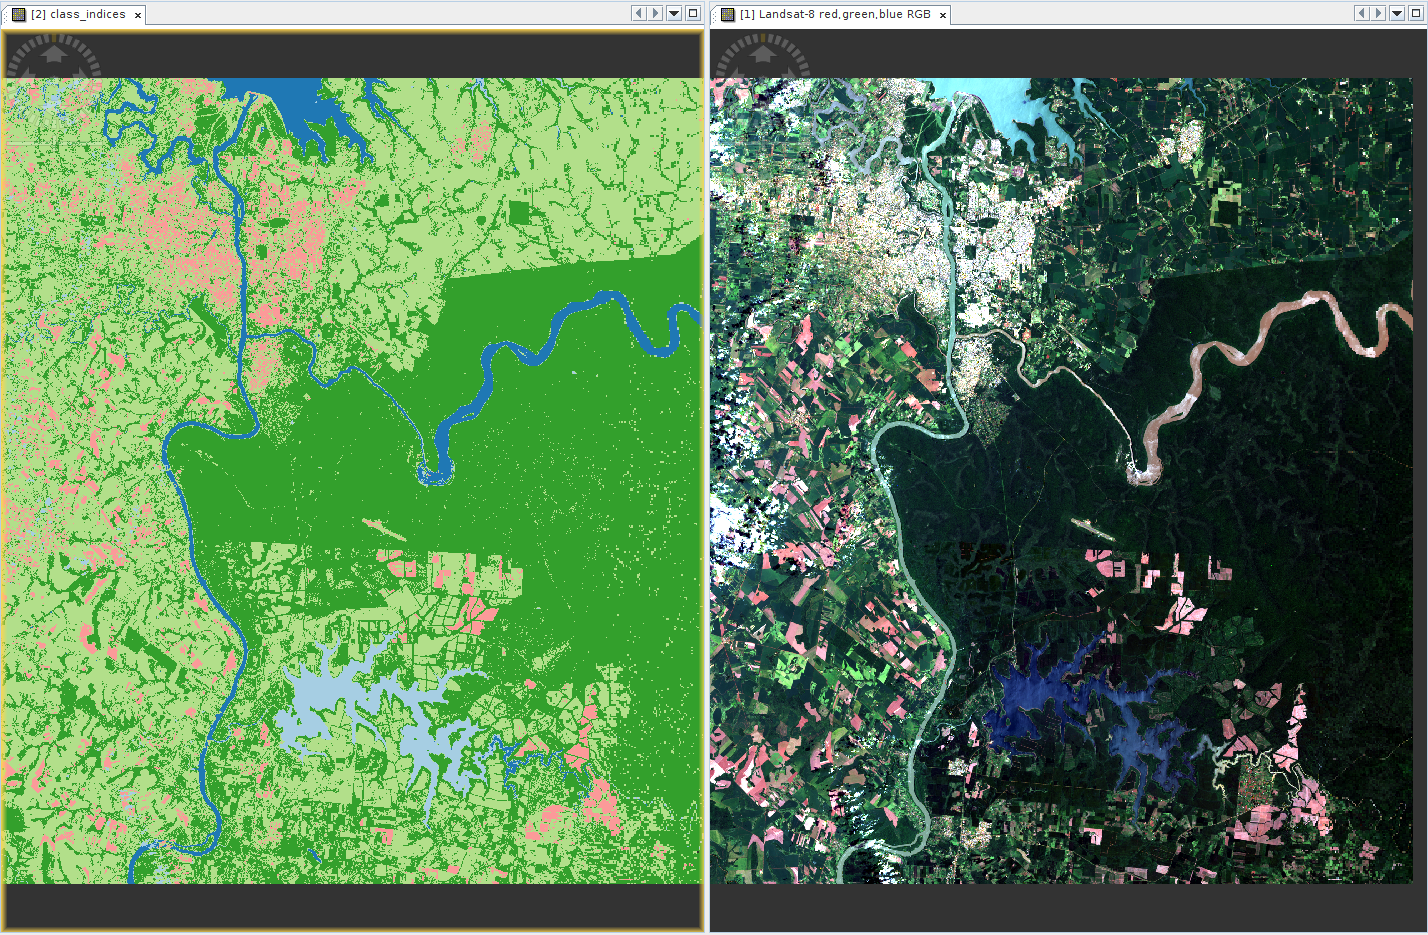
\includegraphics[width=0.7\textwidth]{fig:reclass.png}
    \caption{Imagen reclasificada junto a la imagen en color real.}
    \label{fig:resclass}
\end{figure}

Es posible obtener en la pestaña de \menu{Colour manipulation} el porcentaje de cada clase espectral dentro de la imagen en la columna \emph{Frequency}.

\section{Parámetros de clasificación}

Para mejorar la clasificación obtenida es posible cambiar cuatro parámetros en la pestaña \menu{Processing parameters}

\begin{itemize}
  \item \emph{Number of clusters}: El número de clases espectrales en la que se clasificará la imagen.
  \item \emph{Number of iterations}: El número de veces que se repetirá el proceso de k-means antes de detenerlo si no hay convergencia.
  \item \emph{Random seed}: La semilla que se utiliza para asignar de forma aleatoria las clases iniciales.
  \item \emph{Source band names}: Las bandas que se utilizarán para la clasificación. Si no se selecciona ninguna se utilizaran todas.
\end{itemize}

\section{Exportar visualización}

En el SNAP es posible exportar la vista como imagen para utilizar en otro software. Para ello dirijase a \menu{File > Export > Other > View as image}. Selecciona luego si quiere exportar la región que está viendo (\emph{View region}) o toda la imagen (\emph{Full scene}) y el formato de archivo (Figura \ref{fig:vista}).

\begin{figure}[h!]
    \centering
    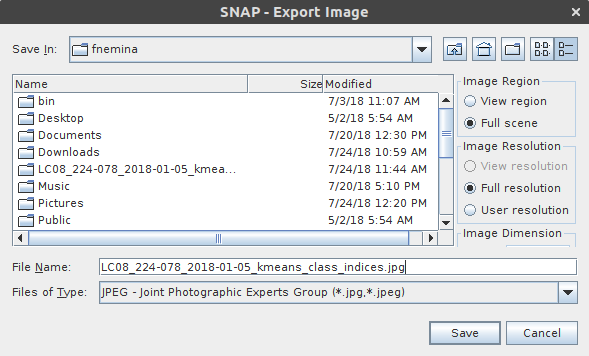
\includegraphics[width=0.5\textwidth]{fig:vista.png}
    \caption{Herramienta para exportar la vista de la imagen.}
    \label{fig:vista}
\end{figure}

Es posible en este caso mantener la georreferenciación eligiendo el formato de archivo \emph{GeoTIFF - TIFF with geo-location}.

En el caso de querer exportar la vista como KMZ debe primero reproyectar la imagen a coordenadas geográficas. En este caso deberá volver a hacer la asignación de colores a cada clase espectral. Luego elija la herramienta \menu{File > Export > Other > View as Google Earth KMZ}.


\section{Actividad práctica}

\begin{enumerate}
  \item Identifique en la imagen las clases que podría asignar a una categoría de uso y cobertura u otra.
  \item Que categorías de uso y cobertura son las que más se confunden dentro de la imagen.
  \item Clasifique la imagen con los siguientes Parámetros
  \begin{table}[h]
  \centering
  \begin{tabular}{cccl}
  \toprule
  Number of clusters & Number of iterations & Random seed & Source band name \\ \midrule
  7                  & 30                   & 31415       & Todas            \\
  14                 & 30                   & 31415       & Todas            \\
  14                 & 30                   & 198674      & Todas            \\
  28                 & 30                   & 31415       & Todas            \\
  28                 & 60                   & 31415       & Todas            \\
  14                 & 30                   & 31415       & blue,green,red   \\
  14                 & 30                   & 31415       & red,nir,swir1    \\ \bottomrule
  \end{tabular}
  \end{table}
  \item ¿Que sucede con la clasificación al aumentar el número de clusters? ¿Y al aumentar el número de iteraciones?
  \item A mismo número de clusters ¿qué bandas conviene utilizar: \emph{blue, green, red} o \emph{red, nir,swir1}? ¿Puede explicar esto en términos de las coberturas de la imagen?
  \item ¿Que parámetros elegiría para una mejor clasificación de la zona?
\end{enumerate}

Estas preguntas y actividades no serán evaluadas. Su objetivo es discutirlas en el foro de consultas e intercambio de la clase.
